\chapter{Research}


\section{2022}

\subsection{June 2022}

I suspect that powell will keep raising rates, I think that they will level off at 5\%. With the new increase of food production and if gas stays around \$100, its still pretty bad for inflation costs. As inflation continues to rise, the prices will eventually go up, less chickens and agriculture products (bad harvest this year).

So I think inflation will hover around 9\% year over year and rates the benchmark rate will hit around 4\%, buy bonds at this point.

Can buy some for rrsp at 6\% or 7\% yield.

https://www.vanguard.ca/en/advisor/products/products-group/etfs/VLB

\section{Green Hydrogen}
After reading the articles from \cite{goldman_sachs_hydrogen_2022} I believe that green hydrogen will be essentially to fully reach zero emissions.

We still need planes, fuel that can do heavy loads for trucking, hydrogen is very verstaile and I believe will do quite well.

One company \index{WATR.V} (Current Water Technologies), is going into the green hydrogen market in an interesting way. They are producing a technology to generate green hydrogen from wastewater, it makes a lot of sense to me. On another note, they reported record sales of 1.5 million just for january and feburary, the likelyhood of this company needing to raise more money soon is unlikely.

Also, they are expanding to aquaculture, if they manage to succeed with their technology, they will do quite well. Their technology can remove toxic ammonia from fishtanks that happen naturally. If their technology can create green hydrogen from waste product, this is a win win for everyone. I think this company is worth holding for a long time.


\begin{figure}[h]
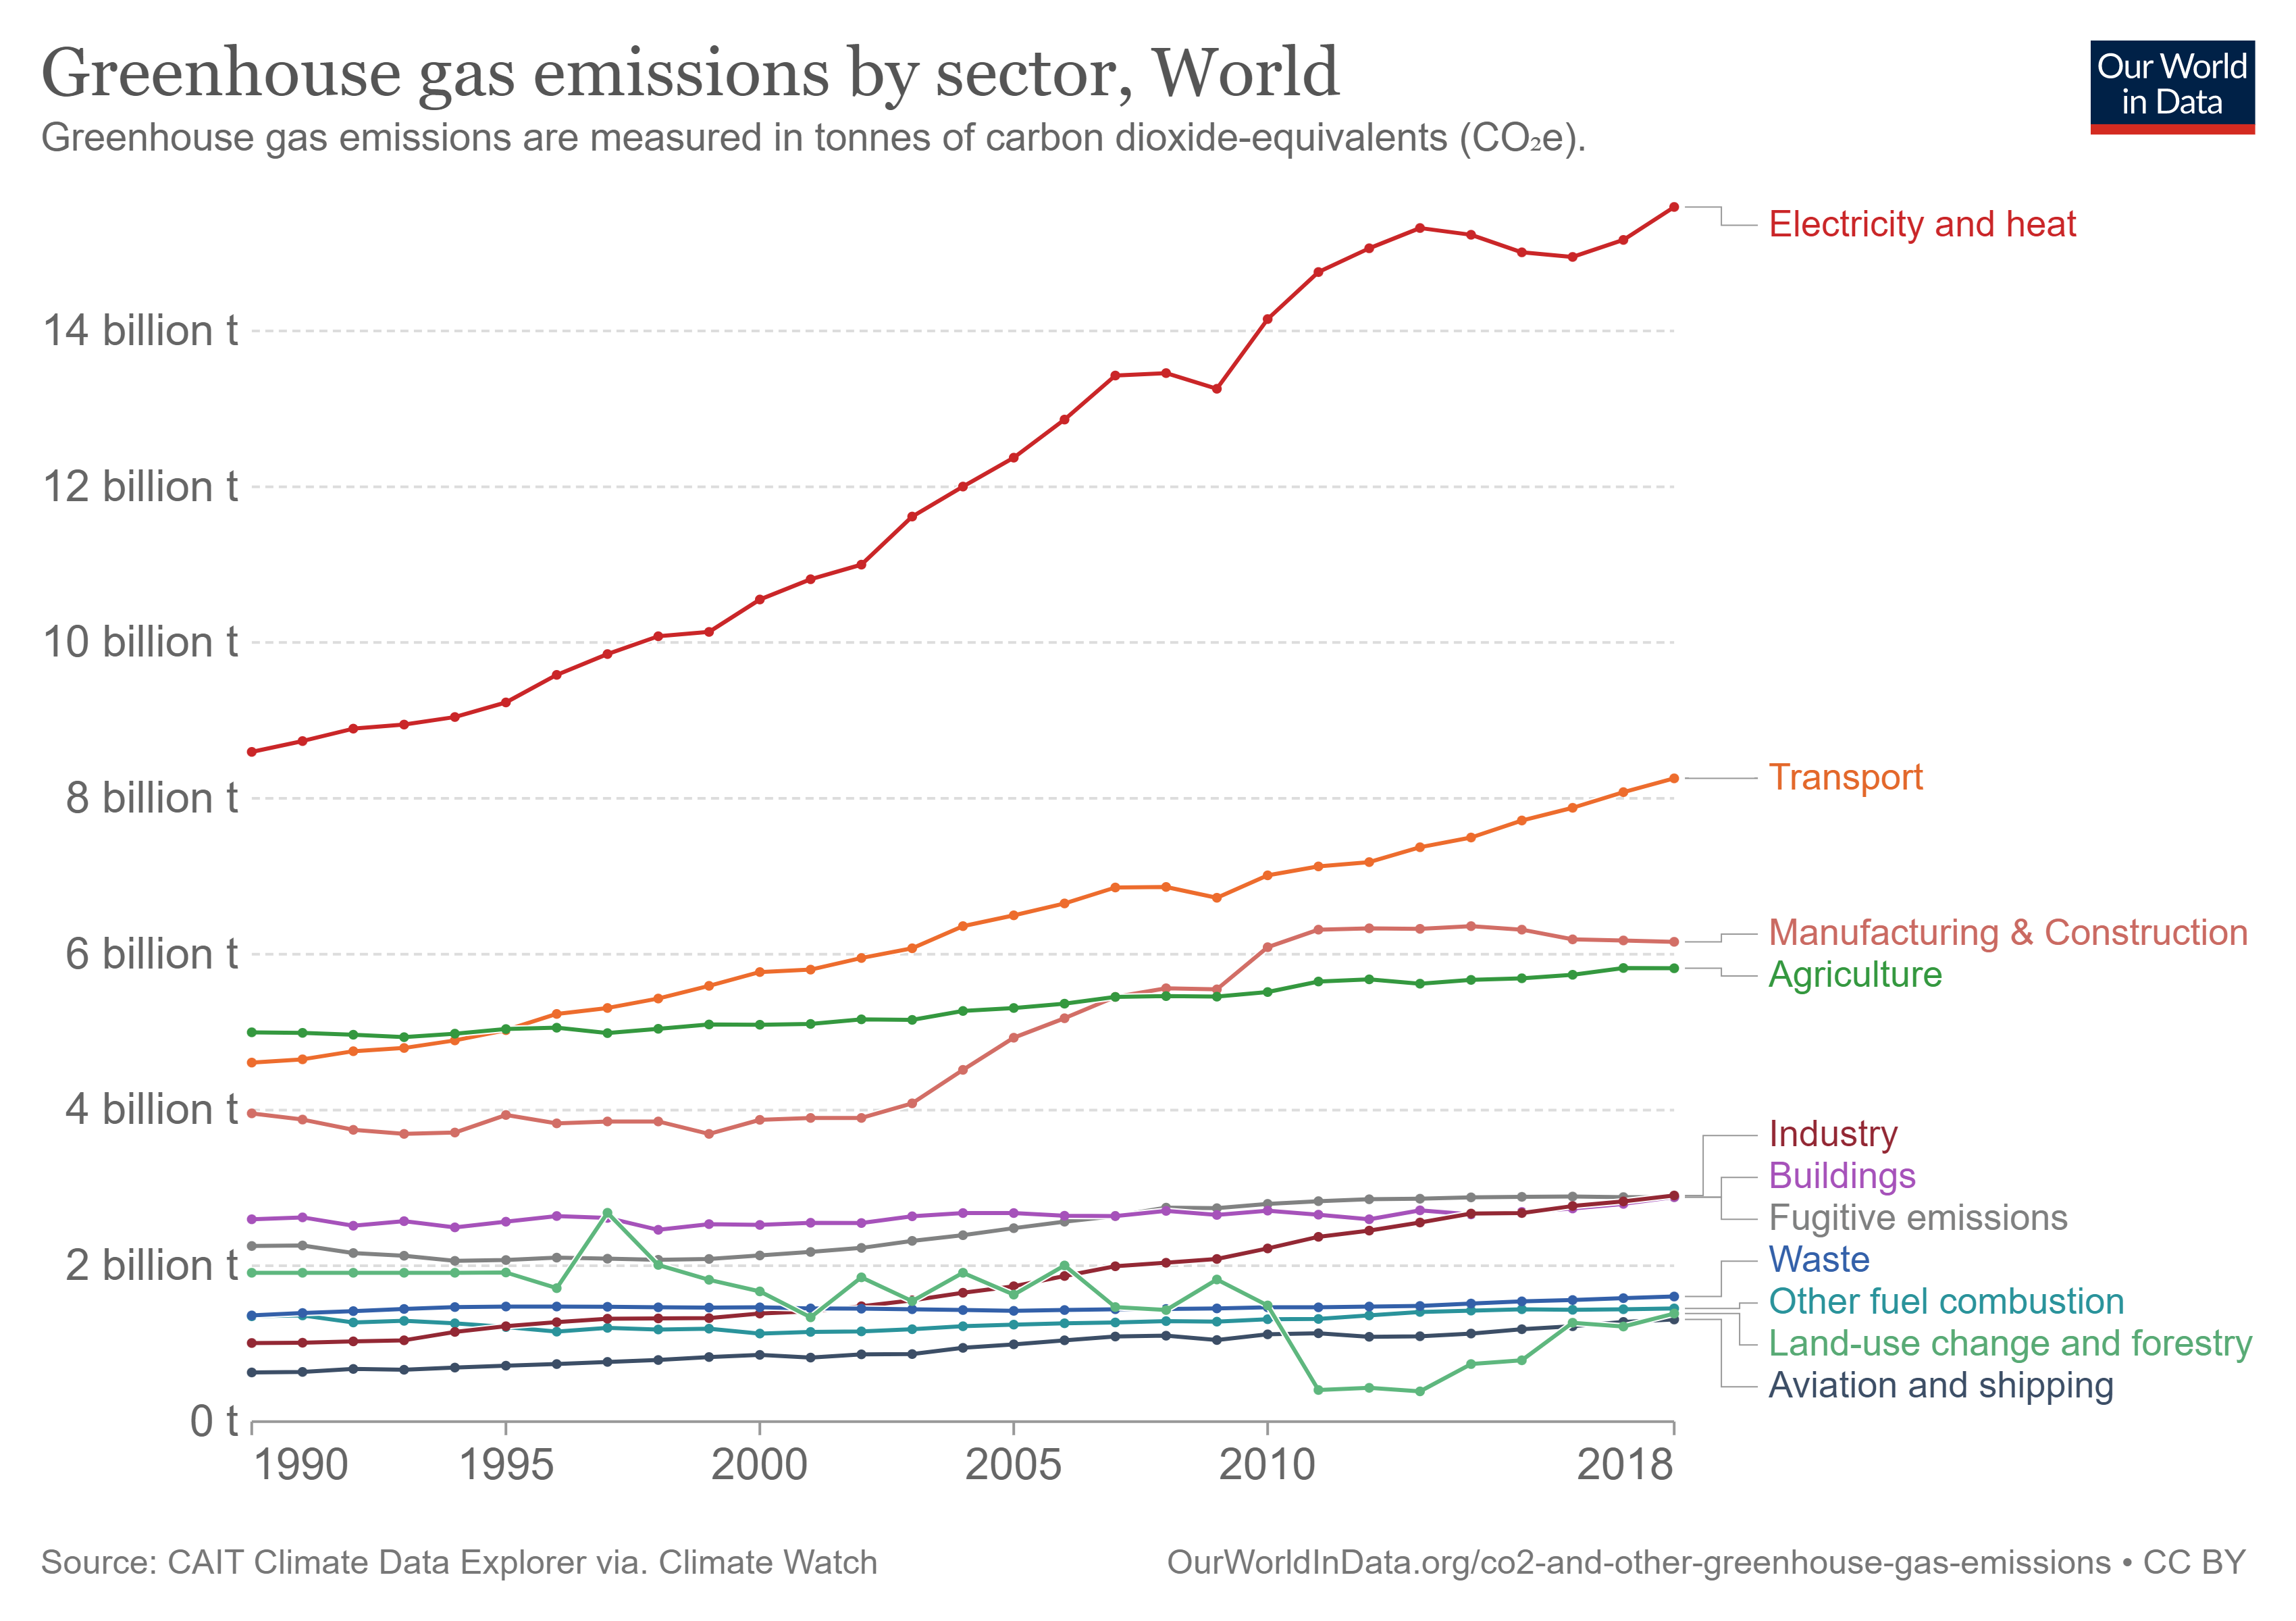
\includegraphics[width=\textwidth]{src/media/ghg-emissions-by-sector.png}
\caption{ghg Emissions by section}
\end{figure}

An estimated 5 trillion dollar for aquaculture alone \cite{goldman_sachs_hydrogen_2022} to reach net zero by 2050, this would imply that we require hydrogen for shipping, transportation, etc.


The potential of green hydrogen for is immense \cite{shipping_green_hydrogen}, for shipping it is an essential server. Companies like \index{ZIM} have already committed to using greener LNG, hydrogen is an natural extension of this.

From the water way technologies (\index{WATR.V}

Independent testing of the ESD system has demonstrated its capabilities. The tests targeted 85\% removal of specific compounds added separately to tap water. The target was achieved in all cases. \cite{cwti_esd}

Why Electro-static Deionization? 
\begin{itemize}
    \item Reduce TDS
    \item High removal efficiencies
    \item High water recovery
    \item No chemical additives
    \item Low maintenance
    \item Low energy consumption
\end{itemize}


\begin{blockquote}
CWTI’s AmmEL–H2 technology has the potential to be one of the world’s most environmentally and economically beneficial hydrogen technologies. It not only produces green hydrogen; it also simultaneously removes toxic ammonia from wastewater. As the AmmEL–H2 system benefits from two revenue streams, this process is an important alternative to traditional electrolyzers that are used only to produce hydrogen gas \cite{ctwi_green_hydrogen}.
\end{blockquote}

\section{Fertilizer and CleanTech}

If the technology is as good as advertised, perhaps it just was not applicable until now, but given the latest new releases and their ability to generate green hydrogen. I believe its worth holding until 0.90 cents and forever in the tsfa accounts. Expected to hit a high amount under tax exemption, I believe with the canada water agency in 2022 good things are ahead for water investments.

Also trudeau pumping 12 billion into the "cleantech" space, there are not that many cleantech companies out there, but who wants to partner with the government, they have too much say in how things are run, and have their own agency that can change every 5 years.


 \begin{displayquote}
Customers prefer our regenerative products because they are made from natural mineral sources which are essential to the plant but do not leach into groundwater like conventional products. KSPC’s potash is an integral part of our blends and this LOI further establishes our long-term relationship and commitment to building the best soil health products possible - commented EarthRenew’s CEO, Keith Driver.
    \end{displayquote}
    
    
More research from the government of Canada's \cite{climate_change_2030_emissions} indicates support for fertilizer management which includes using organic and mineral fertilizer, EarthRenew fertilizer counts as organic which should be a huge plus. Also with the \$170 per ton carbon tax, Earthrenew should be able to grow faster by leveraging waste product, they should have a more friendly process.


\begin{blockquote}
Moving towards a circular economy can also increase the value of waste emissions through transforming raw material into fertilizers and renewable energy \cite{climate_change_2030_emissions}. EarthRenew plan to take waste and convert it to tangible fertilizer is incredible, aiming to hold for 5 years.
\end{blockquote}

The climate report from government of canada suggests that hydrogen production plants are similar in nature to oil refineries \cite{climate_change_2030_emissions}. Earthrenew having plants in Alberta is excellent.


\begin{figure}[h]
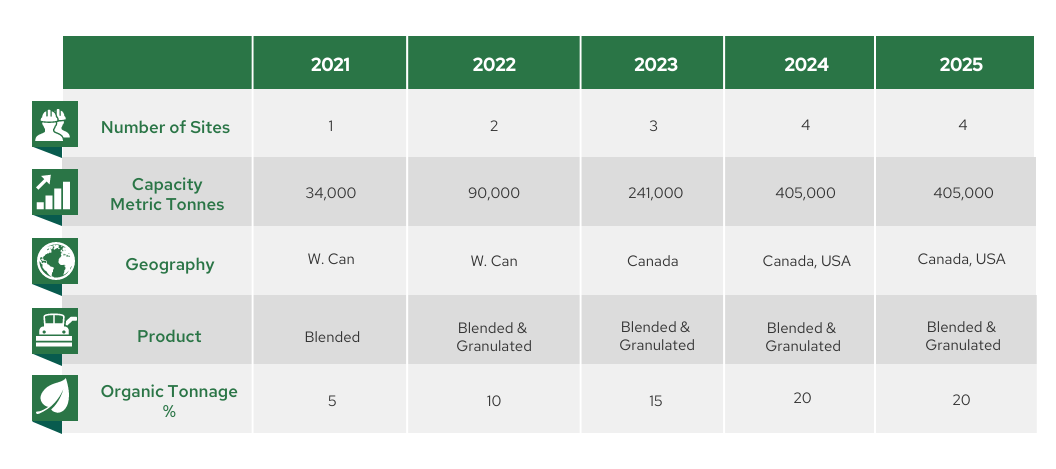
\includegraphics[width=\textwidth]{src/media/63894524-04fe-485b-a801-736431092c3c-e1633360733920.png}
\caption{Growth plan for earth renew}
\end{figure}

Selling their fertilizer along with the planned reduction of 30\% of emissions of fertilizer production in canada \cite{climate_change_2030_emissions}, it is very likely earth renew will get a lot of government support and do quite well. Based on their new releases they seem to be on track if not slightly behind.


\begin{blockquote}
The Government of Canada will continue to drive climate innovation by providing additional funding to
trial pre-commercial clean technologies and de-risk large-scale pilot projects critical to net-zero
transitions. Actions will be taken to enhance the Canadian climate innovation ecosystem to promote the
scale-up of clean tech companies and to coordinate efforts in strategic areas where it can yield major
emissions reduction \cite{climate_change_2030_emissions}. 
\end{blockquote}


\chapter{Valuations}

\section{Earthrenew}
Government of canada already funding case studies for erth.

Essentially the government is subsiding unproven companies like cielo, and/or helping fund earth renew, incredibly likely that earthrenew would qualify for free money.

With the degradation of land \cite{the_guardian_degraded_2022}, we need to start to feeding the land again. The industrialization of agriculture must give back to the soil and store carbon in the soil again.

As for price target, if earthrenew manages to scale production to 241,000, and 405000, would expect a valuation of 10 times pe.

With fertilizer prices at 900 (expect this range for a few years until russia blows over), thats about 

\begin{equation}
  x = 241000*900*0.30*10 = 650700000
\end{equation}

So valuation of 650 million, if they manage to hit 405000, expect 1 billion dollar market cap, and the regenerative properties are very useful for storing carbon, so can expect this premium even if the company earns less than 0.30 margin (probably higher because lower cost inputs at the moment).

\begin{equation}
  x = 405000*900*0.30*10 = 1093500000
\end{equation}


From sales call 24 to 27 million, hot industries, some reports indiciating that it will take 2 or 3 years for the market to go back to normal with the russia invasion, the topsoil erosion cant be fixed overnight

Food yields will go down because of

\begin{itemize}
    \item topsoil erosion
    \item reduction in fertilizer usage
    \item food will cost more because it is more scarce, causing more supply chain disruptions?
    \item value added product, fertilizer is custom formula developed and tested by earthrenew.
    \item explanation to how traditionally fertilizer companies is pretty bad for the environment, very useful nutrients in the rocks
\end{itemize}

\section{Peak Fintech}

according to my estimates 20\% of 345 million is 69 million, maybe 70 million.

15 million + 1 million + 14.39 + 5 million, bare minimum to keep holding is 35 million, assume could be up to 48.3 million, if they can inject 11 million into insurance, likely to be 45 million. 

9 \% due to insurance, mainly in Q2 so assume 1 million revenue, if they got 175 million worth in policies solely in q2, thats insane, about 31.05 million.

For Q2, expecting 17.5 from oil and gas, 7 million from insurance, 36 from consumer goods business

60 to 90 million.

With the consumer goods sector expected to be 50\% in 2022 vs 90\% in 2021.

14,239,776 for 2021 Q1, keeping that in mind.

Results, might as well keep holding 35 million I guess.

\section{ZIM}

I can understand why the stonk price cratered with the shutdown on the china port, but its good for the long run, disruption increases shipping costs with increase profits. For way too long the cost of shipping goods has been too low, and the ability to get things quickly was always extremely fragile.

Expect costs to go up with the shutting down and reopening and the chinese vaccine does not work well.
With all these things considered.

if 93 ships are still chartered for more than one year in March 2023, then the chances of zim continuing to be viable is amazing.

With their increased guidance, \%46 percent dividend expected this year, seems about right to me, think supply chain issues will persist until 2023.

With the new laws banning certain materials from uyghurs, likely to have more supply chain issues.

More covid lockdowns, supply chain issues, south korea truckers, german ports, us ports, export numbers still decent, keep holding. With work shortages cancelling ferries and/or airplanes like in air canada, zim remains a strong hold at least until mid 2023. Can sell before march 2023, to capitalize on big dividend.


\section{FGI}

Boring business that sells sanitaryware and bath furniture, pe is less than 3 and shareholder equtity around 7 million, decently valued compared to the competition, sells like a good buy, will try to bottom fish this company in my rrsp. With rising freight rates, not sure if I should try to play earnings, lets see what the inflation report is like on wedensday, May 11, 2022 and then determine if I should buy according based on my gut feeling.

If the economy keeps going down, fgi will likely tank as sales will decrease, after 284 days, I think the market will recover from the bear market. For fgi in a economic downturn aim for a price of 1.20, ignore pe, as it might be trending down during a recession. With debts of 14.7 million and rising interest rates that should cut into profits, so net income of 5 or 6 million is reasonable.

But with a pe of 2 or 3 with a growing economy, boomers need to upgrade their homes, and with shortage of houses, products should sell, the only matter is margin, shipping rates went down slightly, who knows where production of these products are.

\section{KEI}

Kolibri Global Energy, \$26 million USD in cashflow or \$33 million CAD @ 1.27 divided by 35.6 million shares outstanding is 93 cents a share in cashflow on a \$2.60 stock price that has the potential to really grow further in 2023. 

And thats pegged at \$90 dollars a barrel, if \$110 or \$115 or \$120 barrels of oil that will be insane.


WIth the partial oil ban, I would expect adjusted flow to be, 


33 million / 50 netback = 0.66 million per dollar of oil increase
\begin{figure}
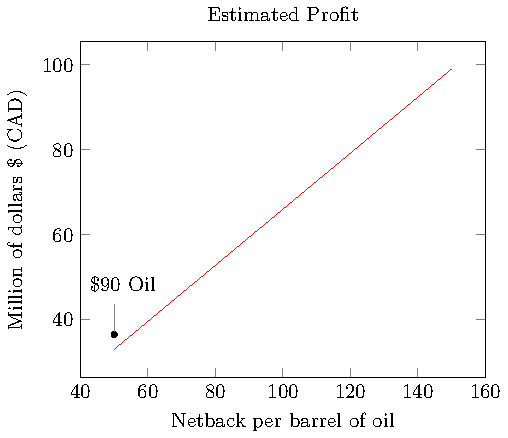
\includegraphics[width=\linewidth]{src/content/images/stonk_research.pdf}
\caption{Kei Estimated profit chart}
\end{figure}

Keep in mind that at 50, the price of oil is \$90, if prices remain at \$110 or \$115, profit should be 46.2 to 49 million cad.

In wells continue to outperform expectations, there is a chance of \$ 50 million or higher netback this year. Will need to compute weighted average of price of oil, Draw a line before Q2 earnings.


\section{Tilray}

With the legalization of cannabis and the rise of interest rates, I Would expect a consolidation in the number of pot companies or the unprofitable companies to get killed off.

Tilray at the current price of \$4.55 has a market cap of about 2 billion, 600 million in assets, all cannabis companies, tilray can likely last a 1 or 2 years before it needs to raise more capital.

By shutting down some facilities and creating synergies they can save money,

Would only buy this at below book value so around 1 or 2 dollars, but likely a big recession at this point.

Given how the competition is getting wrecked, it makes sense, would expect demand of cannabis to stay consistent.


\section{SBSW}

Decent valued gold company, above 10\% dividend yield, in this bear market hoping for 12 to 13\% yield, aiming for 15\% before dumping money in rrsp, with tax free benefits, definitely a solid buy around august 20th, 2022


\section{US Steel}
\subsection{Advantages}

Low PE, dividend very sustainable, decent book value, located in the us, practically no debt. Will 3 Billion cash and a committment to return value to shareholders through buybacks, will consider at low prices.
Planning to buy the week before, 

\subsection{Disadvantages}
low dividend value, prefer stonk buybacks, wait until q3, probably announce more buybacks.

\section{Bloom Health}


If it truly hits 325 million market cap, cad, sell the heck out of it, or the ebita numbers listed below.

As of May 31 2022

As for prices, seems undervalued if they can earn 900k * 3 = 2.7 million or 1.7 million,  with growth and increasing margins, they have secured some funding for 2023 with the extension contract for testing.

\begin{itemize}
    \item Revenue going pretty fast \% 91 in a quarter is no joke
    \item stupid america policies, need an immediate solution for this to prove vaccinations
    \item trying to help out aging workforce.
    \item strong management.
\end{itemize}

Disadvantages

\begin{itemize}
    \item Covid based revenue, covid goes away sooner than expected (within a year or two)
    \item If ebitba milestones are hit, they are expected to hand over cash, but could still be a good thing.
    \item not enough money to meet obligations, expects to meet them their expansion in operations
\end{itemize}

The Company’s current liabilities exceeded its current assets by \$2,971,565 as at March 31, 2022
(September 30, 2021 – \$5,069,219), which includes the fair value of the short-term consideration payable of
\$9,956,467, based on the forecasted timing of payments. As at March 31, 2022, the Company had cash on
hand of \$1,680,144 (September 30, 2021 - \$5,598,296). The Company did not have sufficient cash to meet
its current liabilities as at March 31, 2022, and expects to meet these obligations with expansion in operations through 2022.

Payments to Round Hill

The members of Round Hill are also entitled to receive additional bonus payments (the “Contingent
Consideration”) based upon the achievement of the following milestones:
\begin{itemize}
\item a one-time payment of US\$10,000,000, payable in cash or common shares of the Company, at the
election of the members of Round Hill, upon Round Hill achieving cumulative EBITDA of at least
US\$27,500,000 by December 31, 2023;
\item a one-time payment of US\$20,000,000, payable in cash or common shares of the Company, at the
election of the Company, upon the Company achieving a market capitalization of Cdn\$325,000,000
for thirty consecutive trading days prior to December 31, 2023; and
\item a one-time payment of US\$20,000,000, payable in cash or common shares of the Company, at the
election of the members of Round Hill, upon Round Hill achieving cumulative EBITDA of at least
US\$52,500,000 by December 31, 2023.
\end{itemize}


Evaluation, they project 25 to 28 million dollars revenue when revenue went up 91\% in Q2, 16.9M total revenue, 8.4 million in booked revenue, projections 25-28, seems likely they will hit. Almost EBITDA positive.

